\documentclass[ignorenonframetext,]{beamer}
\setbeamertemplate{caption}[numbered]
\setbeamertemplate{caption label separator}{: }
\setbeamercolor{caption name}{fg=normal text.fg}
\beamertemplatenavigationsymbolsempty
\usepackage{lmodern}
\usepackage{amssymb,amsmath}
\usepackage{ifxetex,ifluatex}
\usepackage{fixltx2e} % provides \textsubscript
\ifnum 0\ifxetex 1\fi\ifluatex 1\fi=0 % if pdftex
\usepackage[T1]{fontenc}
\usepackage[utf8]{inputenc}
\else % if luatex or xelatex
\ifxetex
\usepackage{mathspec}
\else
\usepackage{fontspec}
\fi
\defaultfontfeatures{Ligatures=TeX,Scale=MatchLowercase}
\fi
% use upquote if available, for straight quotes in verbatim environments
\IfFileExists{upquote.sty}{\usepackage{upquote}}{}
% use microtype if available
\IfFileExists{microtype.sty}{%
\usepackage{microtype}
\UseMicrotypeSet[protrusion]{basicmath} % disable protrusion for tt fonts
}{}
\newif\ifbibliography
\usepackage{longtable,booktabs}
\usepackage{caption}
% These lines are needed to make table captions work with longtable:
\makeatletter
\def\fnum@table{\tablename~\thetable}
\makeatother

% Prevent slide breaks in the middle of a paragraph:
\widowpenalties 1 10000
\raggedbottom

\AtBeginPart{
\let\insertpartnumber\relax
\let\partname\relax
\frame{\partpage}
}
\AtBeginSection{
\ifbibliography
\else
\let\insertsectionnumber\relax
\let\sectionname\relax
\frame{\sectionpage}
\fi
}
\AtBeginSubsection{
\let\insertsubsectionnumber\relax
\let\subsectionname\relax
\frame{\subsectionpage}
}

\setlength{\parindent}{0pt}
\setlength{\parskip}{6pt plus 2pt minus 1pt}
\setlength{\emergencystretch}{3em}  % prevent overfull lines
\providecommand{\tightlist}{%
\setlength{\itemsep}{0pt}\setlength{\parskip}{0pt}}
\setcounter{secnumdepth}{0}
% Some style additions.
% RS09022015

% Set the logo.
\pgfdeclareimage[height=0.8cm, width=0.8cm]{logo}{logo.png}
%\logo{\pgfuseimage{logo}\vspace{260pt}}
\logo{\pgfuseimage{logo}}

% Some style settings.
\usetheme{Madrid}
%\usefonttheme{serif}
\usecolortheme{beaver}

% Set additional fields.
\institute[]{\href{https://github.com/bwv988}{https://github.com/bwv988}}

% Further beamer settings.
\setbeamertemplate{navigation symbols}{}
% Some style additions.
% RS09022015

\usepackage{color}
\usepackage{graphicx}
\usepackage{subcaption}
\usepackage{mathtools}
\usepackage{grffile}
\newcommand{\mat}[1]{\mathbf{#1}}
\newcommand{\expt}[1]{\mathbb{E}({#1})}
\newcommand{\hvec}[1]{\hat{\underline{#1}}}
\renewcommand{\vec}[1]{\underline{#1}}

\newcommand{\FIXME}[1]{\noindent{\color{red} FIXME: #1}
}

\newcommand{\HIGHLIGHT}[1]{\noindent{\color{blue}#1}}

\newcommand{\orange}[1]{\textcolor{orange}{#1}}


\DeclarePairedDelimiter\floor{\lfloor}{\rfloor}

\title{CF Tutorial}
\subtitle{Some Notes on Collaborative Filtering}
\author{Ralph Schlosser}
\date{February 2017}

\begin{document}
\frame{\titlepage}

\begin{frame}{Overview}

\begin{itemize}
\tightlist
\item
  Introduction
\item
  Model-based Collaborative Filtering
\item
  Alternating Least Squares: Intuition
\end{itemize}

\end{frame}

\begin{frame}{Introduction}

\begin{itemize}
\tightlist
\item
  Want to predict user ratings for movies which they haven't rated.
\item
  This can be achieved with \HIGHLIGHT{Collaborative Filtering}.
\item
  CF is not \emph{one} algorithm, it's a broad set of different
  techniques.
\item
  Here: Model-based approach using
  \HIGHLIGHT{Alternating Least Squares}.
\end{itemize}

\begin{longtable}[]{@{}lllll@{}}
\toprule
Users & Movie 1 & Movie 2 & Movie 3 & \ldots{}\tabularnewline
\midrule
\endhead
User 1 & \orange{?} & 5.9 & 2.6 & \ldots{}\tabularnewline
User 2 & 1.4 & 5.8 & \orange{?} & \ldots{}\tabularnewline
User 3 & 1.5 & 5.8 & \orange{?} & \ldots{}\tabularnewline
\ldots{} & \ldots{} & \ldots{} & \ldots{} & \ldots{}\tabularnewline
\bottomrule
\end{longtable}

\end{frame}

\begin{frame}{Model-based Collaborative Filtering}

\begin{itemize}
\item
  Have a \emph{sparse} and usually large matrix
  \(\mathbf{R} \in \mathbb{R}^{u \times v}\) of user ratings.
\item
  \(u\) - Number of users (rows)
\item
  \(v\) - Number of movies (columns)
\item
  \(R_{ij}\) - Rating of user \(i\) for movie \(j\).
\item
  Example:
\end{itemize}

\[
\mathbf{R} = 
\begin{pmatrix}
2.2 & 2.7 &  7.7  & 2.9 &  3.3\\
? & ? & 2.6 & 1.2 & 8.9\\
7.0 & ? & 3.5 & 0.7 & 2.1\\
9.1 & 0.6 & ? & 1.8 & ?\\
? & ? & 7.4 & 3.1 & 5.9
\end{pmatrix}
\]

\end{frame}

\begin{frame}{Alternating Least Squares: Intuition}

\begin{itemize}
\tightlist
\item
  Model-based: Try to uncover \HIGHLIGHT{latent factors} that model the
  data.
\item
  Can be achieved through approximate matrix decomposition:
  \(\mathbf{R} \approx \mathbf{U} \times \mathbf{V}^{T}\)
\end{itemize}

\begin{center}
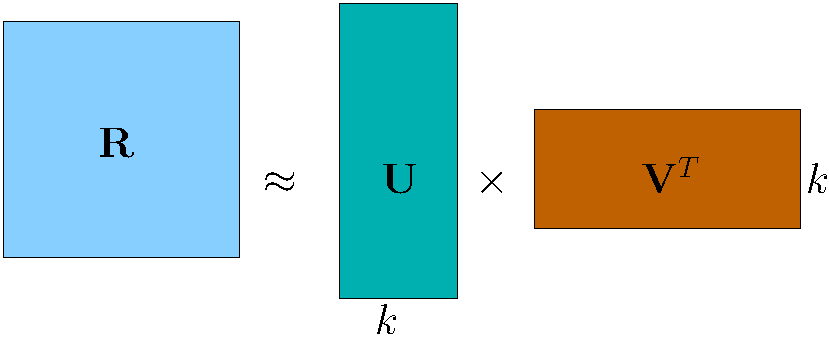
\includegraphics[scale=0.5]{fig/mat_decomp.pdf}
\end{center}

\begin{itemize}
\tightlist
\item
  The \(k\) columns in \(\mathbf{U}\) and \(\mathbf{V}^{T}\) correspond
  to the latent, i.e. \emph{unobserved} factors.
\item
  \orange{ALS}: Approximate \(\mathbf{U}\) and \(\mathbf{V}\) through
  linear regression.
\end{itemize}

\end{frame}

\begin{frame}{Links}

\FIXME{Add links}

\end{frame}

\end{document}
